\documentclass[11pt,twoside]{article}

\usepackage[utf8]{inputenc} % encoding
\usepackage[T1]{fontenc} % encoding

\usepackage[
authordate,
natbib,
backend=biber,
doi=false,
isbn=false,
url=false,
noibid=true
]{biblatex-chicago} % citation package

% natbib style commands
\renewcommand*{\nameyeardelim}{\addcomma\space}
% \newcommand*{\citep}{\parencite}
% \newcommand*{\citet}{\textcite}
\newcommand*{\citefoot}{\footcite}
\newcommand*{\citefull}{\fullcite}
\newcommand*{\citeno}{\nocite}
% \renewcommand*{\cite}{\textcite}

\addbibresource{reference.bib}%

\usepackage{fullpage} % This shrink the margins of the document

\usepackage{enumerate} % customized enumerator

\usepackage{url} % for url and hyperlink

\usepackage{graphicx} % extended graphic package

\usepackage{amsmath} % For equation*, align .....etc.
\usepackage{amsthm} % For theorem environments
\theoremstyle{plain}
\newtheorem{theorem}{Theorem}[section]
\newtheorem{proposition}{Proposition}[section]
\newtheorem{lemma}{Lemma}[section]
\newtheorem{conjecture}{Conjecture}[section]
\newtheorem{algorithm}{Algorithm}[section]
\newtheorem{corollary}{Corollary}[theorem]
\newtheorem{observation}{Observation}[section]
\theoremstyle{definition}
\newtheorem{definition}{Definition}[section]
\theoremstyle{remark}
\newtheorem*{remark}{Remark}
\newtheorem*{note}{Note}
\newtheorem*{claim}{Claim}
\newtheorem{case}{Case}
\newtheorem{example}{Example}


\usepackage{lineno}   % For line numbers in draft
  \linenumbers
  \makeatletter
\newcommand*\patchAmsMathEnvironmentForLineno[1]{%
  \expandafter\let\csname old#1\expandafter\endcsname\csname #1\endcsname
  \expandafter\let\csname oldend#1\expandafter\endcsname\csname end#1\endcsname
  \renewenvironment{#1}%
     {\linenomath\csname old#1\endcsname}%
     {\csname oldend#1\endcsname\endlinenomath}}%
\newcommand*\patchBothAmsMathEnvironmentsForLineno[1]{%
  \patchAmsMathEnvironmentForLineno{#1}%
  \patchAmsMathEnvironmentForLineno{#1*}}%
\AtBeginDocument{%
\patchBothAmsMathEnvironmentsForLineno{equation}%
\patchBothAmsMathEnvironmentsForLineno{align}%
\patchBothAmsMathEnvironmentsForLineno{flalign}%
\patchBothAmsMathEnvironmentsForLineno{alignat}%
\patchBothAmsMathEnvironmentsForLineno{gather}%
\patchBothAmsMathEnvironmentsForLineno{multline}%
}

\usepackage[toc,page]{appendix} % appendix

\usepackage{setspace} % for onehalfspacing
\onehalfspacing

\usepackage[usenames, dvipsnames]{color} % for color names
\newcommand{\green}[1]{\textcolor{green}{[Note: #1]}}
\newcommand{\red}[1]{\textcolor{red}{[Note: #1]}}
%\newcommand{\green}[1]{\textcolor{green}{}}              % use this to turn off comment
%\newcommand{\red}[1]{\textcolor{red}{}}                  % use this to turn off comment

\usepackage[para,online,flushleft]{threeparttable} % complicated tables


\title{This is a title\footnote{Here are some acknowledgements.}}
\author{
  <%= Settings::FIRSTNAME %> <%= Settings::MIDDLENAME %> <%= Settings::LASTNAME %>\footnote{<%= Settings::ADDRESS %> <%= Settings::CITY %> <%= Settings::STATE %> <%= Settings::ZIPCODE %>, <%= Settings::PHONENUMBER %> \protect\url{<%= Settings::EMAIL %>}}\\
  <%= Settings::DEPARTMENTNAME %>, <%= Settings::UNIVERISITYNAME %>
  %\and
  %FirstName2 LastName2\footnote{Address, Phone Number \protect\url{email2@email.com}}\\
  %Department Name, University Name
}
\date{\today}

\graphicspath{ {figures/} }
\sloppy

\begin{document}

\maketitle

\begin{abstract}
\textsc{Preliminary and incomplete. Please do not distribute without permission.} \\

Some abstract text here. Some abstract text here. Some abstract text here. Some abstract text here.
Some abstract text here. Some abstract text here. Some abstract text here. Some abstract text here.
Some abstract text here. Some abstract text here. Some abstract text here. Some abstract text here.
Some abstract text here. Some abstract text here. Some abstract text here. Some abstract text here.
Some abstract text here. Some abstract text here. Some abstract text here. Some abstract text here.
Some abstract text here. Some abstract text here. Some abstract text here. Some abstract text here.
Some abstract text here. Some abstract text here. Some abstract text here. Some abstract text here.
Some abstract text here. Some abstract text here. Some abstract text here. Some abstract text here.
Some abstract text here. Some abstract text here. Some abstract text here. Some abstract text here.

\vspace{20pt}

\noindent \scriptsize{\textbf{JEL Classification: (some classification codes here)}}

\noindent \scriptsize{\textbf{Keywords: (some keywords here)}}


\end{abstract}



\newpage

\section{Introduction} % (fold)
\label{sec:introduction}

Some introduction here. Some introduction here. Some introduction here. Some introduction here.\footnote{Some footnote text here.}
Some introduction here. Some introduction here. Some introduction here. Some introduction here.
Some introduction here. Some introduction here. Some introduction here. Some introduction here.
Some introduction here. Some introduction here. Some introduction here. Some introduction here.
Some introduction here. Some introduction here. Some introduction here. Some introduction here.
Some introduction here. Some introduction here. Some introduction here. Some introduction here.
Some introduction here. Some introduction here. Some introduction here. Some introduction here.
Some introduction here. Some introduction here. Some introduction here. Some introduction here.
Some introduction here. Some introduction here. Some introduction here. Some introduction here.

Some introduction here. Some introduction here. Some introduction here. Some introduction here.\red{here is some red notes.}
Some introduction here. Some introduction here. Some introduction here. Some introduction here.
Some introduction here. Some introduction here. Some introduction here. Some introduction here.\green{testing}
Some introduction here. Some introduction here. Some introduction here. Some introduction here.
Some introduction here. Some introduction here. Some introduction here. Some introduction here.
Some introduction here. Some introduction here. Some introduction here. Some introduction here.
Some introduction here. Some introduction here. Some introduction here. Some introduction here.
Some introduction here. Some introduction here. Some introduction here. Some introduction here.
Some introduction here. Some introduction here. Some introduction here. Some introduction here.

% section introduction (end)

\section{Citation Demo}
\label{sec:Citation Demo}

\citet{Smith2008} says blah blah blah.

\citeauthor{Smith2008} mention blah blah blah in \citeyear{Smith2008}.

\citep{Smith2008}

\citefull{Smith2008}

\citefoot{Smith2008}

\citeno{Smith2008}

\cite{Smith2008}


\section{Another Section} % (fold)
\label{sec:another_section}

Refer to Section \ref{sec:introduction}.

\citet{Smith2008} says blah blah blah. \citeauthor{Smith2008} also mention blah blah blah.

Some text here. Some text here. Some text here. Some text here.
Some text here. Some text here. Some text here. Some text here.
Some text here. Some text here. Some text here. Some text here.

\url{http://www.google.com}

Some text here. Some text here. Some text here. Some text here.
Some text here. Some text here. Some text here. Some text here.
Some text here. Some text here. Some text here. Some text here.

\colorbox{red}{This is highlighted text.}

Some text here. Some text here. Some text here. Some text here.
Some text here. Some text here. Some text here. Some text here.
Some text here. Some text here. Some text here. Some text here.
Some text here. Some text here. Some text here. Some text here.
Some text here. Some text here. Some text here. Some text here.
Some text here. Some text here. Some text here. Some text here.


\fcolorbox{blue}{white}{This is framed text.}

Some text here. Some text here. Some text here. Some text here.
Some text here. Some text here. Some text here. Some text here.
Some text here. Some text here. Some text here. Some text here.


\noindent{\color{MidnightBlue} \rule{\linewidth}{0.5mm} }

\begin{itemize}
\color{ForestGreen}
\item Firts item
\item Second item
\end{itemize}


\noindent{\color{Rhodamine} \rule{\linewidth}{0.5mm} }

Some text here. Some text here. Some text here. Some text here.
Some text here. Some text here. Some text here. Some text here.
Some text here. Some text here. Some text here. Some text here.


Blah Blah Blah is proved \citep{Lee2009}.


Some text here. Some text here. Some text here. Some text here.
Some text here. Some text here. Some text here. Some text here.
Some text here. Some text here. Some text here. Some text here.
Some text here. Some text here. Some text here. Some text here.

\begin{enumerate}
  \item item 1
  \item item 2
  \item item 3
\end{enumerate}

Some text here. Some text here. Some text here. Some text here.
Some text here. Some text here. Some text here. Some text here.
Some text here. Some text here. Some text here. Some text here.
Some text here. Some text here. Some text here. Some text here.
Some text here. Some text here. Some text here. Some text here.
Some text here. Some text here. Some text here. Some text here.
Some text here. Some text here. Some text here. Some text here.

\begin{enumerate}[(a)]
  \item item 1
  \item item 2
  \item item 3
\end{enumerate}

Some text here. Some text here. Some text here. Some text here.
Some text here. Some text here. Some text here. Some text here.
Some text here. Some text here. Some text here. Some text here.
Some text here. Some text here. Some text here. Some text here.
Some text here. Some text here. Some text here. Some text here.
Some text here. Some text here. Some text here. Some text here.
Some text here. Some text here. Some text here. Some text here.

\begin{itemize}
  \item item 1
  \item item 2
  \item item 3
\end{itemize}

Some text here. Some text here. Some text here. Some text here.
Some text here. Some text here. Some text here. Some text here.
Some text here. Some text here. Some text here. Some text here.
Some text here. Some text here. Some text here. Some text here.
Some text here. Some text here. Some text here. Some text here.
Some text here. Some text here. Some text here. Some text here.

\begin{description}
  \item[item name 1] item 1
  \item[item name 2] item 2
  \item[item name 3] item 3
\end{description}

Some text here. Some text here. Some text here. Some text here.
Some text here. Some text here. Some text here. Some text here.
Some text here. Some text here. Some text here. Some text here.


\subsection{Some Subsection}
\label{sub:some_subsection}


Some text here. Some text here. Some text here. Some text here.
Some text here. Some text here. Some text here. Some text here.
Some text here. Some text here. Some text here. Some text here.
Some text here. Some text here. Some text here. Some text here.
Some text here. Some text here. Some text here. Some text here.
Some text here. Some text here. Some text here. Some text here.
Some text here. Some text here. Some text here. Some text here.
Some text here. Some text here. Some text here. Some text here.

\begin{table}[ht]
\centering
\caption{\small{Simple table title}}\label{tab:some_simple_table_label}
\begin{tabular}{lcccc}
  \hline
 & column 1 & column 2 & column 3 \\
  \hline
  row 1 & 1          & 4          & 7 \\
  row 2 & 2          & 5          & 8 \\
  row 3 & 3          & 6          & 9 \\
   \hline
\end{tabular}
\end{table}


Some text here. Some text here. Some text here. Some text here.
Some text here. Some text here. Some text here. Some text here.
Some text here. Some text here. Some text here. Some text here.
Some text here. Some text here. Some text here. Some text here.
Some text here. Some text here. Some text here. Some text here.
Some text here. Some text here. Some text here. Some text here.
Some text here. Some text here. Some text here. Some text here.
Some text here. Some text here. Some text here. Some text here.

\begin{table}[ht]
\centering
\begin{threeparttable}
\caption{\small{Some table title}}\label{tab:some_table_label}
\begin{tabular}{lcccc}
  \hline
 & column 1 & column 2 & column 3 \\
  \hline
  row 1 & 1\tnote{1} & 4          & 7 \\
  row 2 & 2          & 5          & 8 \\
  row 3 & 3          & 6\tnote{2} & 9 \\
   \hline
\end{tabular}
\begin{tablenotes}
\item[1] \footnotesize{Table notes here} \\
\item[2] \footnotesize{Table notes here} \\
\end{tablenotes}
\end{threeparttable}
\end{table}

% subsection some_subsection (end)


\subsection{Another Subsection}
\label{sub:another_subsection}

Refering to subsection \ref{sub:some_subsection}.

Refering to table \ref{tab:some_table_label}.

Some text here. Some text here. Some text here. Some text here.
Some text here. Some text here. Some text here. Some text here.
Some text here. Some text here. Some text here. Some text here.
Some text here. Some text here. Some text here. Some text here.
Some text here. Some text here. Some text here. Some text here.

% subsection anoher_subsection (end)


% section some_section (end)


\section{Section with Theorems} % (fold)
\label{sec:section_with_theorems}

Some text here. Some text here. Some text here. Some text here.
Some text here. Some text here. Some text here. Some text here.
Some text here. Some text here. Some text here. Some text here.
Some text here. Some text here. Some text here. Some text here.
Some text here. Some text here. Some text here. Some text here.

\begin{theorem}
Let $f$ be a function whose derivative exists in every point, then $f$ is
a continuous function.
\end{theorem}

\begin{theorem}[Pythagorean theorem]\label{the:pythagorean}
This is a theorema about right triangles and can be summarised in the next
equation
\begin{equation*}
  x^2 + y^2 = z^2
\end{equation*}
\end{theorem}

And a consequence of theorem \ref{the:pythagorean} is the statement in the next
corollary.

\begin{corollary}
There's no right rectangle whose sides measure 3cm, 4cm, and 6cm.
\end{corollary}

You can reference theorems such as \ref{the:pythagorean} when a label is assigned.

\begin{lemma}
Given two line segments whose lengths are $a$ and $b$ respectively there is a
real number $r$ such that $b=ra$.
\end{lemma}

\begin{proposition}
  some text here
\end{proposition}

\begin{definition}[Fibration]
A fibration is a mapping between two topological spaces that has the homotopy lifting property for every space $X$.
\end{definition}

Some text here. Some text here. Some text here. Some text here.
Some text here. Some text here. Some text here. Some text here.
Some text here. Some text here. Some text here. Some text here.

\setcounter{case}{0}
\begin{case}[Case Name]
This statement is a case.
\end{case}

\begin{case}[Another Case Name]
This statement is another case.
\end{case}

Some text here. Some text here. Some text here. Some text here.
Some text here. Some text here. Some text here. Some text here.
Some text here. Some text here. Some text here. Some text here.
Some text here. Some text here. Some text here. Some text here.
Some text here. Some text here. Some text here. Some text here.
Some text here. Some text here. Some text here. Some text here.




\setcounter{example}{0}
\begin{example}[Example Name]
This statement is an example.
\end{example}

\begin{example}[Another Example Name]
This statement is another example.
\end{example}


Some text here. Some text here. Some text here. Some text here.
Some text here. Some text here. Some text here. Some text here.
Some text here. Some text here. Some text here. Some text here.
Some text here. Some text here. Some text here. Some text here.
Some text here. Some text here. Some text here. Some text here.
Some text here. Some text here. Some text here. Some text here.


\begin{lemma}\label{lem:some_lemma_label}
Given two line segments whose lengths are $a$ and $b$ respectively there
is a real number $r$ such that $b=ra$.
\end{lemma}

\begin{proof}[Proof of lemma \ref{lem:some_lemma_label}]
To prove it by contradiction try and assume that the statemenet is false,
proceed from there and at some point you will arrive to a contradiction.
\end{proof}


\setcounter{case}{0}
\begin{case}
This statement is a case.
\end{case}

\begin{case}
This statement is another case.
\end{case}

\begin{remark}
This statement is true, I guess.
\end{remark}

\begin{note}
This statement is true.
\end{note}


% section section_with_theorems (end)


\section{Yet Another Section} % (fold)
\label{sec:yet_another_section}

Some text here. Some text here. Some text here. Some text here.
Some text here. Some text here. Some text here. Some text here.

Some text here. Some text here. Some text here. Some text here.
Some text here. Some text here. Some text here. Some text here.
Some text here. Some text here. Some text here. Some text here.

Some text here. Some text here. Some text here. Some text here.
Some text here. Some text here. Some text here. Some text here.
Some text here. Some text here. Some text here. Some text here.
Some text here. Some text here. Some text here. Some text here.


\begin{equation} \label{equ:regresion}
  Y_{i,g} = \alpha + X_{i,g} \beta + \rho_{g} e_{i,g}
\end{equation}

Some text here. Some text here. Some text here. Some text here.
Some text here. Some text here. Some text here. Some text here.
Some text here. Some text here. Some text here. Some text here.
Some text here. Some text here. Some text here. Some text here.
Some text here. Some text here. Some text here. Some text here.

Refer to equation \ref{equ:regresion}.


\begin{equation} \label{equ:regresion2}
  e_{i,g} = \frac{Y_{i,g}}{\rho_{g}} - \frac{\alpha}{\rho_{g}} - \frac{X_{i,g} \beta}{\rho_{g}}
\end{equation}


Some text here. Some text here. Inline math ($y = mx + c$)
Some text here. Some text here.
Some text here. Some text here. Some text here. Some text here.
Some text here. Some text here. Some text here. Some text here.
Some text here. Some text here. Some text here. Some text here.
Some text here. Some text here. Some text here. Some text here.

\begin{align*}
x&=y           &  w &=z              &  a&=b+c\\
2x&=-y         &  3w&=\frac{1}{2}z   &  a&=b\\
-4 + 5x&=2+y   &  w+2&=-1+w          &  ab&=cb
\end{align*}


Some text here. Some text here. Some text here. Some text here.
Some text here. Some text here. Some text here. Some text here.
Some text here. Some text here. Some text here. Some text here.
Some text here. Some text here. Some text here. Some text here.


\begin{figure}[ht!]
  \caption{A picture of $Y$}
  \centering
    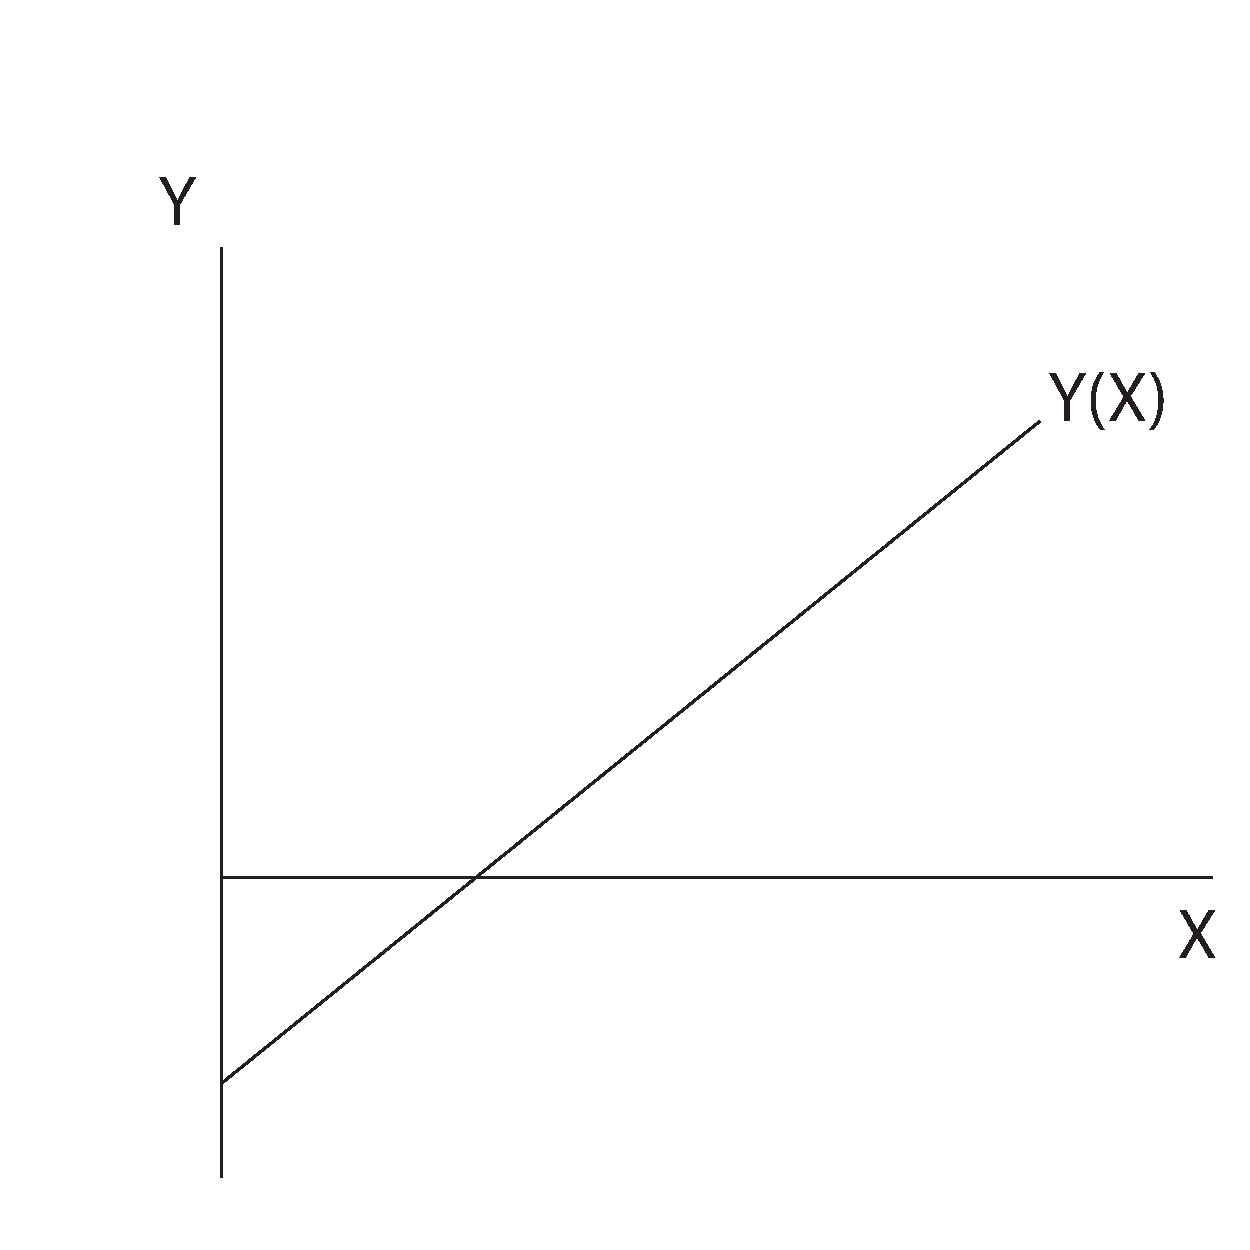
\includegraphics[width=0.5\textwidth]{sample-figure}
\end{figure}


Refer to equation \ref{equ:regresion2}.


% subsection yet_another_section (end)


\section{Conclusion} % (fold)
\label{sec:conclusion}

Some conclusion here. Some conclusion here. Some conclusion here. Some conclusion here.
Some conclusion here. Some conclusion here. Some conclusion here. Some conclusion here.
Some conclusion here. Some conclusion here. Some conclusion here. Some conclusion here.
Some conclusion here. Some conclusion here. Some conclusion here. Some conclusion here.
Some conclusion here. Some conclusion here. Some conclusion here. Some conclusion here.
Some conclusion here. Some conclusion here. Some conclusion here. Some conclusion here.
Some conclusion here. Some conclusion here. Some conclusion here. Some conclusion here.
Some conclusion here. Some conclusion here. Some conclusion here. Some conclusion here.
Some conclusion here. Some conclusion here. Some conclusion here. Some conclusion here.


% section conclusion (end)

\newpage

\printbibliography

\newpage

\appendix
\renewcommand{\thesection}{Appendix \Roman{section}}
\renewcommand{\thesubsection}{Appendix \Roman{section}(\roman{subsection})}

\section{Some Appendix} % (fold)
\label{sec:some_appendix}

Some text here. Some text here. Some text here. Some text here.
Some text here. Some text here. Some text here. Some text here.
Some text here. Some text here. Some text here. Some text here.
Some text here. Some text here. Some text here. Some text here.
Some text here. Some text here. Some text here. Some text here.

% section some_appendix (end)

\section{Another Appendix} % (fold)
\label{sec:another_appendix}

Some text here. Some text here. Some text here. Some text here.
Some text here. Some text here. Some text here. Some text here.
Some text here. Some text here. Some text here. Some text here.
Some text here. Some text here. Some text here. Some text here.
Some text here. Some text here. Some text here. Some text here.

% section another_appendix (end)


\end{document}
